\section{Implementation HGF coupling}

If we assume that a cortical column consists of units (i.e., sub-populations of neurons), one for each computational step, then the computations for \textsf{VAPE coupling} as well as for \textsf{VOPE coupling} could be implemented as sketched in Figure 1.

\begin{figure}[h]
	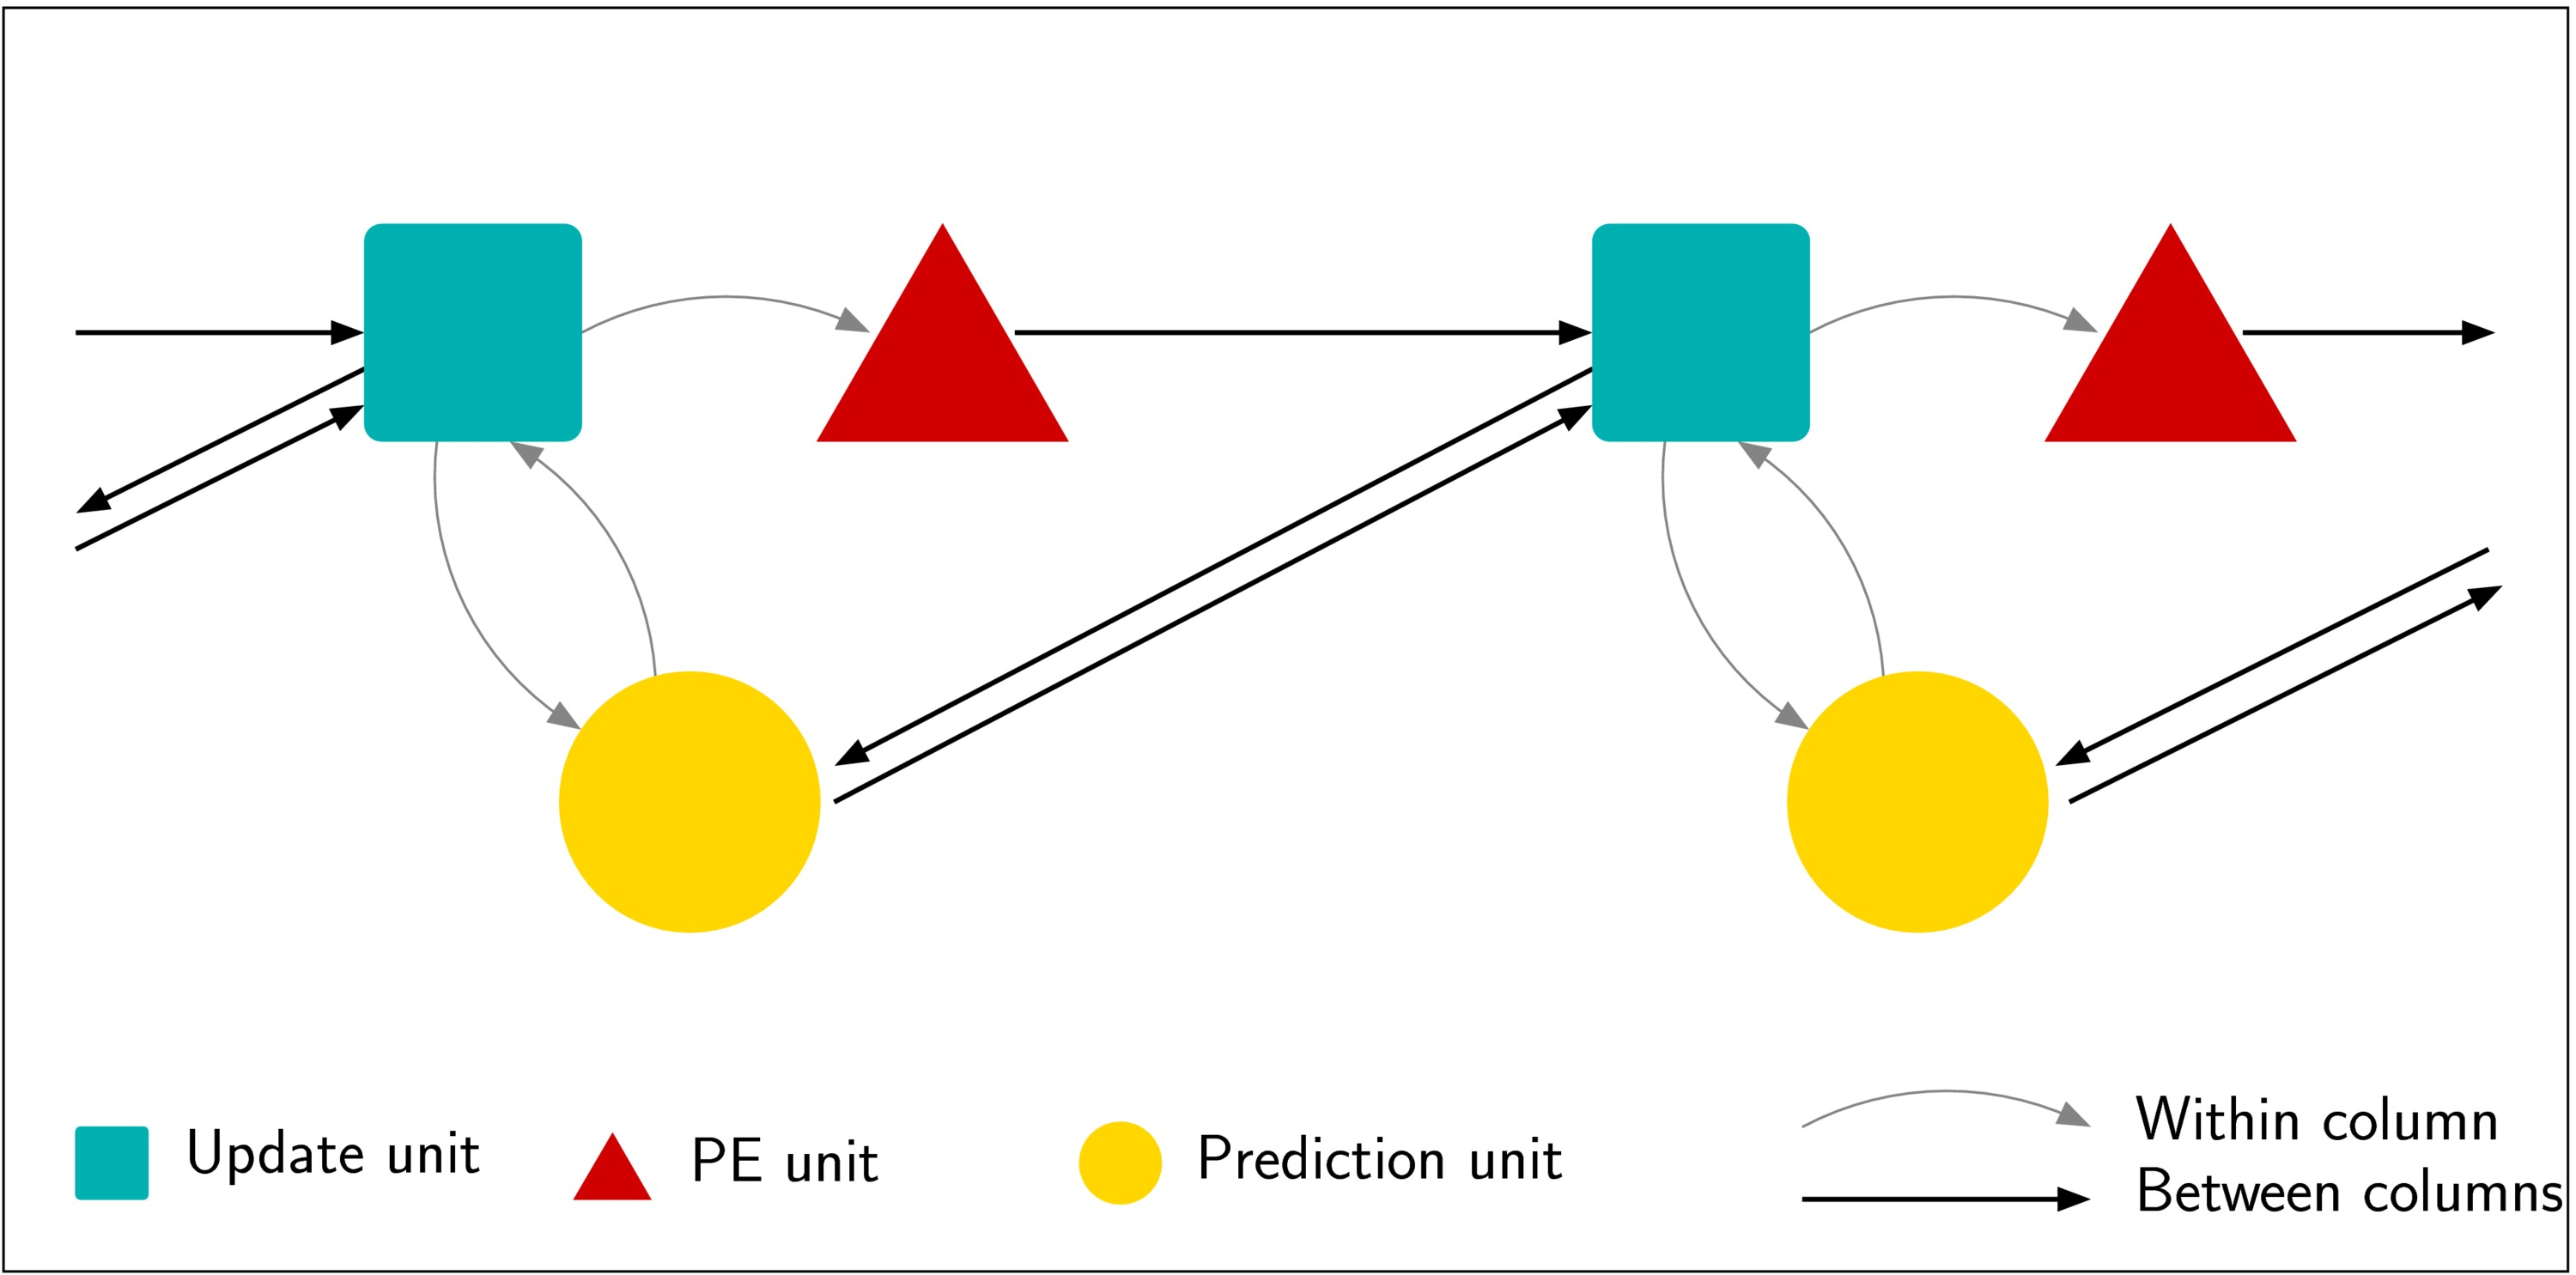
\includegraphics[width = \textwidth]{figures/impl/fig.jpeg}
	\caption{Example implementation of the coupling between cortical columns in the HGF. Figure shows two cortical columns that could be coupled to each other via VAPE or VOPE coupling. In each case, the messages passed along the connections and the computations within the nodes would differ according to the equations presented in the previous chapters.}
\end{figure}

A few points to note here:
\begin{itemize}
\item In this implementation, we assume that the estimated volatility, $\nu_i^{k}$, is computed within the \textsf{Prediction} unit. This is motivated by the equations presented above and the fact that this unit receives information about the updated quantities (posterior means and precisions) from the level above.
\item Similarly, the only unit that needs to know the value of a node's tonic learning rate, $\omega_i$, is the \textsf{Prediction} unit. Therefore, this parameter could be implemented in terms of self-connections or interneurons within than neuronal population.
\item One very annoying arrow in this picture is the one from the \textsf{Prediction} unit of one node to the \textsf{Update} unit of its parent node. This is annoying, because it violates the classical assumptions that while top-down connections signal predictions, bottom-up connections would only signal prediction errors. Due to the update equations in the HGF, however, any given parent node needs access to the predicted precision from its child node to perform an update. To avoid this arrow, we could also assume that the \textsf{Prediction} unit sends the predicted precision to the \textsf{PE} unit of the same node, which then sends this quantity up to the \textsf{Update} unit of the parent node. However, this seems more complicated for two reasons: First, the \textsf{PE} unit doesn't actually need this quantity to perform its computation. Secondly, the PE is computed only somewhat after the prediction of the current trial (which is already computed after the previous trial). Thus, the two signals would be sent up at different times.
\end{itemize}
%\newpage